\documentclass[professionalfont,dvipdfmx,cjk,xcolor=dvipsnames,envcountsect,notheorems,12pt]{beamer}
% * 16:9 のスライドを作るときは、aspectratio=169 を documentclass のオプションに追加する
% * 印刷用の配布資料を作るときは handout を documentclass のオプションに追加する
%   (overlay が全て一つのスライドに出力される)

\usepackage{tikz}
\usetikzlibrary{positioning}
\usepackage{newtxmath}
\usepackage{pxjahyper}% しおりの文字化け対策 (なくても良い)
\usepackage{amsmath,amssymb,amsfonts,amsthm,ascmac,cases,bm,pifont}
\usepackage{graphicx}
\usepackage{url} \usepackage{bussproofs}
\usepackage{etex}
\usepackage{color}
\usepackage[all,cmtip]{xy}
\usepackage{mathtools}

\makeatletter
\def\underbracket{%
       \@ifnextchar [ %
              {\@underbracket}%
              {\@underbracket [\@bracketheight]}%
}
\def\@underbracket[#1]{%
       \@ifnextchar [ %
              {\@under@bracket[#1]}%
               {\@under@bracket[#1][0.4em]}%
}
\def\@under@bracket[#1][#2]#3{%\message {Underbracket: #1,#2,#3}
       \mathop {%
              \vtop {%
                     \m@th \ialign {%
                            ##\crcr $\hfil \displaystyle {#3}\hfil $%
                   \crcr \noalign %
                            {\kern 3\p@ \nointerlineskip }%
                            \upbracketfill {#1}{#2}
                   \crcr \noalign %
                            {\kern 3\p@ }%
                     }%
              }%
       }%
       \limits%
}
\def\upbracketfill#1#2{%
       $\m@th \setbox \z@ \hbox {$\braceld$}
       \edef\@bracketheight{\the\ht\z@}\bracketend{#1}{#2}
       \leaders \vrule \@height #1 \@depth \z@ \hfill 
       \leaders \vrule \@height #1 \@depth \z@ \hfill%
       \bracketend{#1}{#2}$%
}
\def\bracketend#1#2{\vrule height #2 width #1\relax}
\def\overbracket{\@ifnextchar [ {\@overbracket} {\@overbracket
[\@bracketheight]}}
\def\@overbracket[#1]{\@ifnextchar [ {\@over@bracket[#1]}
{\@over@bracket[#1][0.3em]}}
\def\@over@bracket[#1][#2]#3{%\message {Overbracket: #1,#2,#3}
\mathop {\vbox {\m@th \ialign {##\crcr \noalign {\kern 3\p@
\nointerlineskip }\downbracketfill {#1}{#2}
                              \crcr \noalign {\kern 3\p@ }
                              \crcr  $\hfil \displaystyle {#3}\hfil $%
                              \crcr} }}\limits}
\def\downbracketfill#1#2{$\m@th \setbox \z@ \hbox {$\braceld$}
                  \edef\@bracketheight{\the\ht\z@}\downbracketend{#1}{#2}
                  \leaders \vrule \@height #1 \@depth \z@ \hfill
                  \leaders \vrule \@height #1 \@depth \z@ \hfill
\downbracketend{#1}{#2}$}
\def\downbracketend#1#2{\vrule depth #2 width #1\relax}
\makeatother

% スライドのテーマ
\usetheme{sumiilab}
% ベースになる色を指定できる
%\usecolortheme[named=Magenta]{structure}
% 数式の文字が細くて見難い時は serif の代わりに bold にしましょう
%\mathversion{bold}

%% ===============================================
%% スライドの表紙および PDF に表示される情報
%% ===============================================

%% 発表会の名前とか(省略可)
%\session{研究室ゼミ}
%% スライドのタイトル
\title{Formal Verifications of \mbox{Call-by-Need and Call-by-Name} Evaluations with \mbox{Mutual Recursion}}
%% 必要ならば、サブタイトルも
%\subtitle{研究の進捗報告}
%% 発表者のお名前
\author{Masayuki Mizuno\\Joint work with Eijiro Sumii}
%% 発表者の所属([] 内は短い名前)
\institute[Tohoku University Sumii-Matsuda Laboratory]{Tohoku University}
%\institute[東北大学 住井・松田研]{工学部 電気情報物理工学科\\住井・松田研究室}% 学部生
%\institute[東北大学 住井・松田研]{大学院情報科学研究科 情報基礎科学専攻\\住井・松田研究室}% 院生
%% 発表する日
\date{November 19, 2019}

%% ===============================================
%% 自動挿入される目次ページの設定(削除しても可)
%% ===============================================

%% section の先頭に自動挿入される目次ページ(削除すると、表示されなくなる)
\AtBeginSection[]{
\begin{frame}
  \frametitle{Outline}
  \tableofcontents[sectionstyle=show/shaded,subsectionstyle=show/show/hide]
\end{frame}}
%% subsection の先頭に自動挿入される目次ページ(削除すると、表示されなくなる)
%\AtBeginSubsection[]{
%\begin{frame}
%  \frametitle{アウトライン}
%  \tableofcontents[sectionstyle=show/shaded,subsectionstyle=show/shaded/hide]
%\end{frame}}

%% 現在の section 以外を非表示にする場合は以下のようにする

%% \AtBeginSection[]{
%% \begin{frame}
%%   \frametitle{アウトライン}
%%   \tableofcontents[sectionstyle=show/hide,subsectionstyle=show/show/hide]
%% \end{frame}}
%% \AtBeginSubsection[]{
%% \begin{frame}
%%   \frametitle{アウトライン}
%%   \tableofcontents[sectionstyle=show/hide,subsectionstyle=show/shaded/hide]
%% \end{frame}}

%% ===============================================
%% 定理環境の設定
%% ===============================================

%\setbeamertemplate{theorems}[numbered]% 定理環境に番号を付ける
\theoremstyle{definition}
\newtheorem{definition}{Definition}
\newtheorem{axiom}{Axiom}
\newtheorem{theorem}{Theorem}
\newtheorem{lemma}{Lemma}
\newtheorem{corollary}{Corollary}
\newtheorem{proposition}{Proposition}

%% ===============================================
%% ソースコードの設定
%% ===============================================

\usepackage{listings,jlisting}
%\usepackage[scale=0.9]{DejaVuSansMono}

\definecolor{DarkGreen}{rgb}{0,0.5,0}
% プログラミング言語と表示するフォント等の設定
\lstset{
  language={[Objective]Caml},% プログラミング言語
  basicstyle={\ttfamily\small},% ソースコードのテキストのスタイル
  keywordstyle={\bfseries},% 予約語等のキーワードのスタイル
  commentstyle={},% コメントのスタイル
  stringstyle={},% 文字列のスタイル
  frame=trlb,% ソースコードの枠線の設定 (none だと非表示)
  numbers=none,% 行番号の表示 (left だと左に表示)
  numberstyle={},% 行番号のスタイル
  xleftmargin=5pt,% 左余白
  xrightmargin=5pt,% 右余白
  keepspaces=true,% 空白を表示する
  mathescape,% $ で囲った部分を数式として表示する ($ がソースコード中で使えなくなるので注意)
  % 手動強調表示の設定
  moredelim=[is][\itshape]{@/}{/@},
  moredelim=[is][\color{red}]{@r\{}{\}@},
  moredelim=[is][\color{blue}]{@b\{}{\}@},
  moredelim=[is][\color{DarkGreen}]{@g\{}{\}@},
}

\newcommand{\xtwoheadrightarrow}[2][]{%
  \xrightarrow[#1]{#2}\mathrel{\mkern-14mu}\rightarrow
}

\newcommand{\keyword}[1]{\mathbf{#1}}
\newcommand{\LET}[2]{\keyword{let}~#1~\keyword{in}~#2}
\newcommand{\CIF}[3]{\keyword{if}~#1~\keyword{then}~#2~\keyword{else}~#3}
\newcommand{\VAR}[1]{\keyword{var}~#1}
\newcommand{\LOC}[1]{\keyword{loc}~#1}
\newcommand{\ABS}[1]{\keyword{abs}~#1}
\newcommand{\FUN}[2]{\keyword{fun}~#1\Rightarrow #2}
\newcommand{\LAM}[2]{\lambda #1 .~#2}
\newcommand{\APP}[2]{\keyword{app}~#1~#2}
\newcommand{\CONS}[2]{\keyword{cons}~#1~#2}
\newcommand{\VCONS}[2]{\keyword{vcons}~#1~#2}
\newcommand{\CASE}[4]{\keyword{case}~#1~\keyword{of}~\{#2~#3 \Rightarrow #4\}}
\newcommand{\REC}{\keyword{rec}}
\newcommand{\ARRAY}{\keyword{Array}}
\newcommand{\CREATE}{\keyword{create}}
\newcommand{\AND}{\keyword{and}}
\newcommand{\IN}{\keyword{in}}
\newcommand{\TRUE}{\keyword{true}}
\newcommand{\WHILE}{\keyword{while}}
\newcommand{\DO}{\keyword{do}}
\newcommand{\DONE}{\keyword{done}}
\newcommand{\BVAR}{\keyword{bvar}}
\newcommand{\FVAR}{\keyword{fvar}}
\newcommand{\FULLBETA}{\xrightarrow{\beta}}
\newcommand{\CALLBYVALUE}{\xrightarrow{\mathrm{value}}}
\newcommand{\CALLBYNAME}{\xrightarrow{\mathrm{name}}}
\newcommand{\CALLBYNEED}{\xrightarrow{\mathrm{need}}}
\newcommand{\RTCLOSFULLBETA}{\xtwoheadrightarrow{\beta}}
\newcommand{\RTCLOSCALLBYNAME}{\xtwoheadrightarrow{\mathrm{name}}}
\newcommand{\RTCLOSCALLBYNEED}{\xtwoheadrightarrow{\mathrm{need}}}
\newcommand{\EVALNEED}[4]{\langle \textcolor{HeapBlue}{#1} \rangle \textcolor{TermGreen}{#2} \Downarrow_\mathtt{d} \langle \textcolor{HeapBlue}{#3} \rangle \textcolor{TermGreen}{#4}}
\newcommand{\DIVERGENEED}[2]{\langle \textcolor{HeapBlue}{#1} \rangle \textcolor{TermGreen}{#2}\Uparrow_\mathtt{d}}
\newcommand{\EVALNAMEHEAP}[4]{\langle \textcolor{HeapBlue'}{#1} \rangle \textcolor{TermGreen'}{#2} \Downarrow_\mathtt{m} \langle \textcolor{HeapBlue'}{#3} \rangle \textcolor{TermGreen'}{#4}}
\newcommand{\DIVERGENAMEHEAP}[2]{\langle \textcolor{HeapBlue'}{#1}\rangle \textcolor{TermGreen'}{#2}\Uparrow_\mathtt{m}}
\newcommand{\EVALNAMECLOS}[3]{\{\textcolor{EnvBlue}{#1} \} \textcolor{TermGreen}{#2} \Downarrow_\mathtt{m} \textcolor{ClosBlue}{#3}}
\newcommand{\DIVERGENAMECLOS}[2]{\{\textcolor{EnvBlue}{#1} \} \textcolor{TermGreen}{#2} \Uparrow_\mathtt{m}}
\newcommand{\EVALNAMESUBST}[2]{\textcolor{TermGreen}{#1} \Downarrow_\mathtt{m} \textcolor{TermGreen}{#2}}
\newcommand{\DIVERGENAMESUBST}[1]{\textcolor{TermGreen}{#1} \Uparrow_\mathtt{m}}
\newcommand{\SUBST}[3]{#1[#2\mapsto #3]}
\newcommand{\RCONS}[2]{#1,~#2}
\newcommand{\SIZE}[1]{|#1|}
\newcommand{\NTH}[2]{#1.#2}
\newcommand{\CAT}[2]{#1,~#2}
\newcommand{\SETNTH}[3]{#1[#2\mapsto #3]}
\newcommand\doubleplus{\mathbin{+\kern-1.3ex+\kern0.8ex\!\!}}
\newcommand{\CLOS}[2]{\keyword{cls}(#1,~#2)}
\newcommand{\HGET}[2]{#1(#2)}
\newcommand{\ISOHEAP}[3]{#2 \sim_{#1} #3}
\newcommand{\CORRHEAPHEAP}[3]{#2 \leq_{#1} #3}
\newcommand{\CORRHEAPCLOS}[3]{#2 \leq_{#1} #3}
\newcommand{\CORRHEAPSUBST}[2]{\mathit{let}_{#1}(\textcolor{HeapBlue'}{#2})}
\newcommand{\CORRTERMHEAP}[3]{#2 \sim_{#1} #3}
\newcommand{\CORRTERMCLOS}[4]{#3 \sim_{#1}^{#2} #4}
\newcommand{\CORRTERMSUBSTF}[3]{#2 \sim_{#1} #3}
\newcommand{\CORRTERMSUBST}[4]{\langle \textcolor{HeapBlue'}{#1} \rangle \textcolor{TermGreen'}{#3} \sim_{#2} \textcolor{TermGreen}{#4}}
\newcommand{\SHIFT}[2]{{\uparrow^{#1}}#2}
\newcommand{\REDNAMEHEAP}[4]{\langle #1 \rangle#2\rightarrow_\mathtt{m} \langle #3 \rangle #4}
\newcommand{\REDMULTINAMEHEAP}[4]{\langle \textcolor{HeapBlue'}{#1} \rangle\textcolor{TermGreen'}{#2}\rightarrow_\mathtt{m}^* \langle \textcolor{HeapBlue'}{#3} \rangle \textcolor{TermGreen'}{#4}}
\newcommand{\REDUCIBLENAMEHEAP}[2]{\langle \textcolor{HeapBlue'}{#1} \rangle\textcolor{TermGreen'}{#2}\mathop{\rightarrow_\mathtt{m}}}
\newcommand{\REDMULTINAMESUBST}[2]{\textcolor{TermGreen}{#1}\rightarrow_\mathtt{m}^* \textcolor{TermGreen}{#2}}
\newcommand{\REDUCIBLENAMESUBST}[1]{\textcolor{TermGreen}{#1}\mathop{\rightarrow_\mathtt{m}}}
\newcommand{\lBrack}{\ensuremath{[\![}}
\newcommand{\rBrack}{\ensuremath{]\!]}}

\newcommand*{\aboxed}[2]{%
  \rlap{\boxed{#1#2}}%
  \phantom{\hskip\fboxrule\hskip\fboxsep #1}&\phantom{#2}%
}

%% ===============================================
%% 本文
%% ===============================================
\begin{document}
\frame[plain]{\titlepage}% タイトルページ

\section*{Outline}

\begin{frame}
	\frametitle{Our goals}
	\begin{itemize}
		\item Long-term: formally verified compiler for \mbox{\alert{non-strict} language (e.g. Haskell)}
		\pause
		\item Short-term: formal verification of correspondence between
		\begin{itemize}
			\item Call-by-name {\small [Plotkin 1975 etc.]}:\\High-level specification of \mbox{\alert{non-strict} languages}
			\item Call-by-need {\small [Wadsworth 1971 etc.]}:\\Implementation of \mbox{\alert{non-strict} languages}
		\end{itemize}
	\end{itemize}
\end{frame}

\begin{frame}
	\frametitle{Background 1: non-strict language}
	\Large
	Allows users to define non-strict functions e.g.
	\[\mathtt{const42}~x = \CIF{\TRUE}{42}{x}\]
	\begin{center}
		\begin{minipage}{.55\linewidth}
			\begin{block}{}
				\centering
				$\begin{array}{ll}
					& \mathtt{const42}~(\mathtt{loop}~())\\
					\twoheadrightarrow & 42
				\end{array}$
			\end{block}
		\end{minipage}
	\end{center}
	\flushright{where\quad$\mathtt{loop}~() = 3+\mathtt{loop}~()$}
\end{frame}

\begin{frame}
	\frametitle{Background 2: call-by-name}
	\Large
	Substitute arguments \alert{without} evaluating them
	\[\mathtt{const42}~x = \CIF{\TRUE}{42}{x}\]
	% 数式風に
	% = 値
	\begin{center}
		\begin{minipage}{.85\linewidth}
			\begin{block}{}
				$\begin{array}{ll}
					& \mathtt{const42}~(\mathtt{loop}~())\\
					\visible<2->{\CALLBYNAME & \CIF{\TRUE}{42}{\mathtt{loop}~()}}\\
					\visible<3->{\CALLBYNAME & 42}
				\end{array}$
			\end{block}
		\end{minipage}
	\end{center}
	\flushright{where\quad$\mathtt{loop}~() = 3+\mathtt{loop}~()$}
\end{frame}

\begin{frame}
	% However, call-by-name sometimes needs redundant reductions due to redex duplication.
	% For example, let me evaluate a term (\lambda x.~xx)~(I~I).
	% Although full-beta reduction can evaluate in 3 steps, call-by-name reduction needs 4 steps!
	\frametitle{Problem of call-by-name:\\redundant computations}
	\Large
	\[\mathtt{double}~x=x+x\]
	\begin{center}
		\begin{minipage}{.6\linewidth}
			\begin{block}{}
				$\begin{array}{ll}
					& \mathtt{double}~(3+3) \\
					\pause
					\CALLBYNAME & (3+3)+(3+3) \\
					\pause
					\CALLBYNAME & 6+(3+3) \\
					\pause
					\CALLBYNAME & 6+6 \\
					\pause
					\CALLBYNAME & 12
				\end{array}$
			\end{block}
		\end{minipage}
	\end{center}
\end{frame}

\begin{frame}
	% Therefore, actual implementations reuses the result of evaluation, namely, call-by-need reduction.
	% Its behaviour should correspond with call-by-name.
	\frametitle{Background 3: call-by-need}
	% x + x \emph{where} x = 1 + 2
	\begin{itemize}
		\item Shares values of arguments
			\[\mathtt{double}~x=x+x\]
			\begin{center}
				\begin{minipage}{.8\linewidth}
					\begin{block}{}
						$\begin{array}{ll}
							& \mathtt{double}~(3+3) \\
							\pause
							\CALLBYNEED & x+x\quad\mathit{where}\quad x=3+3 \\
							\pause
							\CALLBYNEED & x+x\quad\mathit{where}\quad x=6 \\
							%				\CALLBYNEED \hspace{1mm}\overbracket[1pt][0.5em]{\hspace{-1mm}\bullet+\hspace{1mm}\underbracket[1pt][0.5em]{\hspace{-1mm}\bullet \qquad \fbox{1+2}\hspace{-0.75em}}}\\
							%				\CALLBYNEED \hspace{1mm}\overbracket[1pt][0.5em]{\hspace{-1mm}\bullet+\hspace{1mm}\underbracket[1pt][0.5em]{\hspace{-1mm}\bullet \qquad \hspace{0.6em}\fbox{3}\hspace{-0.15em}}}\\
							\pause
							\CALLBYNEED & 12
						\end{array}$
					\end{block}
				\end{minipage}
			\end{center}
			\pause
		\item Should correspond with call-by-name
	\end{itemize}
\end{frame}

\begin{frame}
	\frametitle{Challenge: recursion (1/2)}
	\begin{itemize}
		\item Implicit recursion destroys sharing
			\[Y~f=(\lambda x.~f~(x~x))~(\lambda x.~f~(x~x))\]
			$\LET{x=e_x}{x}\quad \Rightarrow\quad Y~(\lambda x.~e_x)$
			\begin{itemize}
				\item Computation of $e_x$ inside $\lambda x$ is repeated
			\end{itemize}
	\end{itemize}
\end{frame}

%\begin{frame}
%	\large
%	\begin{minipage}{\linewidth}
%		\begin{block}{}
%			$\begin{array}{l}
%				{\begin{array}{ll}
%					\phantom{\RTCLOSCALLBYNEED}	& \LET{x=\alert<1>{(\lambda z.~z)~(\lambda y.~x)}}{x~3~4}
%				\end{array}} \\
%				\pause
%				{\begin{array}{rlcl}
%					\CALLBYNEED & x~3~4 & \mathit{where} & x=\alert<2>{(\lambda z.~z)~(\lambda y.~x)} \\
%					\pause
%					\CALLBYNEED & x~3~4 & \mathit{where} & x=\alert<3>{\lambda y.~x} \\
%					\pause
%					\CALLBYNEED & \alert<4>{(\lambda y.~x)}~3~4 & & \\
%					\pause
%					\CALLBYNEED & x~4 & & \\
%					\pause
%					\CALLBYNEED & \alert<6>{(\lambda y.~x)}~4 & & \\
%					\pause
%					\CALLBYNEED & x & &
%				\end{array}}
%			\end{array}$
%		\end{block}
%	\end{minipage}
%\end{frame}
%
%\begin{frame}
%	\frametitle{}
%	{\large $Y~f=(\lambda x.~f~(x~x))~(\lambda x.~f~(x~x))$}
%	\begin{minipage}{\linewidth}
%		\begin{block}{}
%			$\begin{array}{l}
%				{\begin{array}{ll}
%					\phantom{\RTCLOSCALLBYNEED}	& Y~(\lambda x.~\alert<1>{(\lambda z.~z)~(\lambda y.~x)})~3~4 \\
%				\end{array}} \\
%				\pause
%				{\begin{array}{rlcl}
%					\RTCLOSCALLBYNEED & \alert<2>{(\lambda z.~z)~(\lambda y.~x')}~3~4 & \mathit{where} &  f=\lambda x.~\alert<2>{(\lambda z.~z)~(\lambda y.~x)}\\
%					\pause
%					\RTCLOSCALLBYNEED & \alert<3>{(\lambda y.~x')}~3~4 & \mathit{where} &  f=\lambda x.~\alert<3>{(\lambda z.~z)~(\lambda y.~x)}\\
%					\pause
%					\CALLBYNEED & x'~4 & & \\
%					\pause
%					\RTCLOSCALLBYNEED & \alert<5>{(\lambda z.~z)~(\lambda y.~x'')}~4 & & \\
%					\pause
%					\RTCLOSCALLBYNEED & \alert<6>{(\lambda y.~x'')}~4 & & \\
%					\pause
%					\CALLBYNEED & x'' & &
%				\end{array}}
%			\end{array}$
%		\end{block}
%	\end{minipage}
%\end{frame}
%
\begin{frame}
	\frametitle{Challenge: recursion (2/2)}
	\Large
	\begin{itemize}
		\item Explicit recursion requires sophisticated mechanism
			\begin{itemize}
				\item Dependency in small-step semantics\\
					\vspace{-2mm}
					%行間
					{\small [Ariola+ 97]}
					{\large $\begin{array}{lcl}
						E & \vcentcolon\vcentcolon = & \cdots \\
						& | & \LET{D,x=E}{E'[x]} \\
						& | & \LET{x_n=E,D[x,x_n]}{E'[x]} \\
						D[x,x_n] & \vcentcolon\vcentcolon = & x=E[x_1],\cdots,x_{n-1}=E[x_n], D
					\end{array}$}
				\item Fixed point in denotational semantics\\
					\vspace{-2mm}
					{\small [Launchbury 93]}
					{\large $\mu \rho'.~\rho \sqcup (x_1 \mapsto \lBrack e_1 \rBrack_{\rho'}\cdots x_n \mapsto \lBrack e_n \rBrack_{\rho'})$}
			\end{itemize}
	\end{itemize}
\end{frame}

\begin{frame}
	\frametitle{Our results}
	\vspace{-5mm}
	\begin{itemize}
		\item \alert{Simple formal verification} (in Coq) of correspondence among call-by-need and \mbox{3 different styles of call-by-name evaluations} of language with \alert{explicit mutual recursion}
			\begin{itemize}
				\pause
				\item Call-by-need natural semantics
					\pause
					\begin{itemize}
						\item heap-based {\small \mbox{[Launchbury 93]}}
					\end{itemize}
				\pause
				\item Call-by-name natural semantics
					\begin{itemize}
						\pause
						\item heap-based {\small \mbox{[Launchbury 93]}}
						\pause
						\item closure-based {\small (cf. \mbox{[Launchbury 93]})}
						\pause
						\item substitution-based {\small \mbox{[Church 36]}}
					\end{itemize}
			\end{itemize}
		\pause
		\item[$\blacklozenge$] Cf. correspondence with call-by-name denotational semantics {\small \mbox{[Breitner 18]}}
	\end{itemize}
\end{frame}

\begin{frame}
	\frametitle{Proof outline}
	\begin{itemize}
		\item Consists of 3 correspondences
	\end{itemize}
	% 吹き出しにkey:
	\begin{figure}[b]
		\centering
		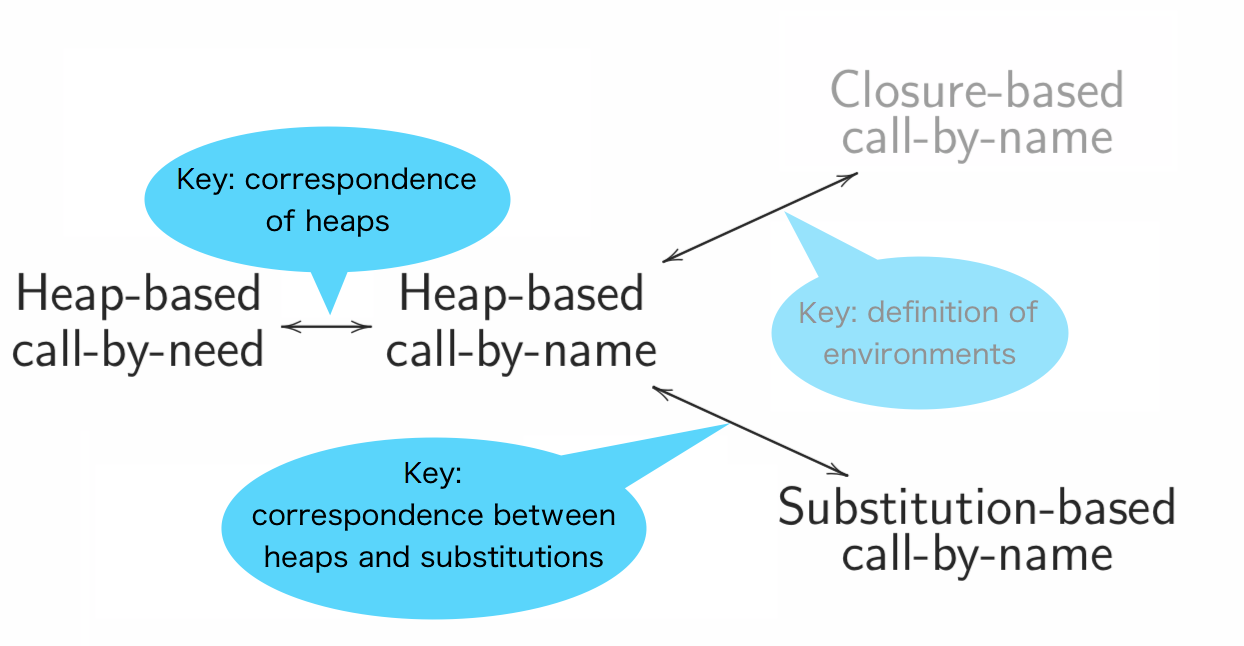
\includegraphics[height=62mm]{correspondences.png}
	\end{figure}
\end{frame}

% 目次を表示させる(section を表示し、subsection は隠す)
\begin{frame}
  \frametitle{Outline}
  \tableofcontents[sectionstyle=show,subsectionstyle=hide]
\end{frame}

%\section{Target language}

%\begin{frame}
%	\frametitle{Heap-based call-by-name semantics (2/2)}
%	\large
%	\fbox{$\DIVERGENAMEHEAP{H}{e}$}
%	\vfill
%	\begin{minipage}{0.45\hsize}
%		\begin{prooftree}
%			\AxiomC{$\DIVERGENAMEHEAP{H}{\NTH{H}{l}}$}
%			\doubleLine
%			\UnaryInfC{$\DIVERGENAMEHEAP{H}{\LOC{l}}$}
%		\end{prooftree}
%	\end{minipage}
%	\begin{minipage}{0.45\hsize}
%		\begin{prooftree}
%			\AxiomC{$\DIVERGENAMEHEAP{H}{e_1}$}
%			\doubleLine
%			\UnaryInfC{$\DIVERGENAMEHEAP{H}{\APP{e_1}{e_2}}$}
%		\end{prooftree}
%	\end{minipage}
%	\begin{prooftree}
%		\AxiomC{$\EVALNAMEHEAP{H_1}{e_1}{H_2}{\ABS{e_0}}$}
%		\AxiomC{$\DIVERGENAMEHEAP{\RCONS{H_2}{e_2}}{\SUBST{e_0}{0}{\LOC{\SIZE{H_2}}}}$}
%		\doubleLine
%		\BinaryInfC{$\DIVERGENAMEHEAP{H_1}{\APP{e_1}{e_2}}$}
%	\end{prooftree}
%	\begin{prooftree}
%		\AxiomC{$\DIVERGENAMEHEAP{\CAT{H_1}{\overline{e}[\forall x\mapsto \LOC{(\SIZE{H_1}+x)}]}}{e[\forall x\mapsto \LOC{(\SIZE{H_1}+x)}]}$}
%		%\AxiomC{$\langle \CAT{H_1}{\overline{e}[\forall x\mapsto \LOC{(\SIZE{H_1}+x)}]} \rangle$}
%		%\noLine
%		%\UnaryInfC{${e[\forall x\mapsto \LOC{(\SIZE{H_1}+x)}]} \Uparrow_d$}
%		\doubleLine
%		\UnaryInfC{$\DIVERGENAMEHEAP{H_1}{\LET{\overline{e}}{e}}$}
%	\end{prooftree}
%\end{frame}

%\begin{frame}
%	\frametitle{Closure-based call-by-name semantics}
%	\Large
%	\begin{itemize}
%		\item Based on environments and closures
%		\item Informally corresponds to denotational semantics [Launchbury 93]
%	\end{itemize}
%	\[\begin{array}{lclcl}
%		c & \in & \textit{Cls} & ::= & \CLOS{E}{e} \\
%		E & \in & \textit{Env} & ::= & \epsilon~|~c :: E~|~(\mu.\overline{e}) \doubleplus E
%	\end{array}\]
%	\large
%	\[\begin{array}{rcl}
%		\HGET{\epsilon}{x} & = & \mbox{undefined} \\
%		\HGET{(c :: E)}{x} & = &
%		\left\{
%		\begin{array}{ll}
%			c & \quad (x=0) \\
%			\HGET{E}{x-1} & \quad (x > 0)
%		\end{array}
%		\right. \\
%		\HGET{((\mu. \overline{e}) \doubleplus E)}{x} & = &
%		\left\{
%		\begin{array}{ll}
%			\CLOS{(\mu. \overline{e}) \doubleplus E}{\NTH{\overline{e}}{x}} & \quad (x<|\overline{e}|) \\
%			\HGET{E}{x-|\overline{e}|} & \quad (x \geq |\overline{e}|)
%		\end{array}
%		\right.
%	\end{array}\]
%\end{frame}
%
%\begin{frame}
%	%\frametitle{Evaluation rules (1/2)}
%	\frametitle{Evaluation rules}
%	\Large
%	\vspace{-5mm}
%	\begin{prooftree}
%		\AxiomC{}
%		\UnaryInfC{$\EVALNAMECLOS{E}{\ABS{e}}{\CLOS{E}{\ABS{e}}}$}
%	\end{prooftree}
%	\begin{prooftree}
%		\AxiomC{$\HGET{\textcolor{EnvBlue}{E}}{x}=\textcolor{ClosBlue}{\CLOS{E_0}{e}}$}
%		\AxiomC{$\EVALNAMECLOS{E_0}{e}{c}$}
%		\BinaryInfC{$\EVALNAMECLOS{E}{\VAR{x}}{c}$}
%	\end{prooftree}
%	\begin{prooftree}
%		\AxiomC{$\EVALNAMECLOS{E}{e_1}{\CLOS{E'}{\ABS{e_0}}}$}
%		\noLine
%		\UnaryInfC{$\EVALNAMECLOS{\CLOS{E}{e_2}::E'}{e_0}{c}$}
%		\UnaryInfC{$\EVALNAMECLOS{E}{\APP{e_1}{e_2}}{c}$}
%	\end{prooftree}
%	\begin{prooftree}
%		\AxiomC{$\EVALNAMECLOS{(\mu. \overline{e}) \doubleplus E}{e}{c}$}
%		\UnaryInfC{$\EVALNAMECLOS{E}{\LET{\overline{e}}{e}}{c}$}
%	\end{prooftree}
%\end{frame}

%\begin{frame}
%	\frametitle{Evaluation rules (2/2)}
%	\Large
%	\begin{prooftree}
%		\AxiomC{$\HGET{\textcolor{EnvBlue}{E}}{x}=\textcolor{ClosBlue}{\CLOS{E_0}{e}}$}
%		\AxiomC{$\DIVERGENAMECLOS{E_0}{e}$}
%		\doubleLine
%		\BinaryInfC{$\DIVERGENAMECLOS{E}{\VAR{x}}$}
%	\end{prooftree}
%	\begin{prooftree}
%		\AxiomC{$\DIVERGENAMECLOS{E}{e_1}$}
%		\doubleLine
%		\UnaryInfC{$\DIVERGENAMECLOS{E}{\APP{e_1}{e_2}}$}
%	\end{prooftree}
%	\begin{prooftree}
%		\AxiomC{$\EVALNAMECLOS{E}{e_1}{\CLOS{E'}{\ABS{e_0}}}$}
%		\noLine
%		\UnaryInfC{$\DIVERGENAMECLOS{\CLOS{E}{e_2}::E'}{e_0}$}
%		\doubleLine
%		\UnaryInfC{$\DIVERGENAMECLOS{E}{\APP{e_1}{e_2}}$}
%	\end{prooftree}
%	\begin{prooftree}
%		\AxiomC{$\DIVERGENAMECLOS{(\mu. \overline{e}) \doubleplus E}{e}$}
%		\doubleLine
%		\UnaryInfC{$\DIVERGENAMECLOS{E}{\LET{\overline{e}}{e}}$}
%	\end{prooftree}
%\end{frame}


%\renewcommand{\EVALNEED}[4]{\langle #1 \rangle #2 \Downarrow_\mathtt{d} \langle #3 \rangle #4}
%\renewcommand{\DIVERGENEED}[2]{\langle #1 \rangle #2\Uparrow_\mathtt{d}}
%\renewcommand{\EVALNAMEHEAP}[4]{\langle #1 \rangle #2 \Downarrow_\mathtt{m} \langle #3 \rangle #4}
%\renewcommand{\DIVERGENAMEHEAP}[2]{\langle #1 \rangle #2\Uparrow_\mathtt{m}}
%\renewcommand{\EVALNAMESUBST}[2]{#1 \Downarrow_\mathtt{m} #2}
%\renewcommand{\DIVERGENAMESUBST}[1]{#1 \Uparrow_\mathtt{m}}

\section{Proof of the correspondences}

\begin{frame}
	\frametitle{Our target language}
	% 見た目違うけど
	\begin{itemize}
		\item $\lambda$-calculus with \mbox{\alert{mutually recursive bindings}}
			\vspace{-7mm}
			\begin{itemize}
				\item Using de Bruijn indices
			\end{itemize}
	\end{itemize}
	\Large
	\[\begin{array}{lclcll}
		x,~l & \in & \textit{Nat} & & \\
		H,~\overline{e} & \in & \alert{\textit{Terms}} \\
		v & \in & \textit{Value} & ::= & \ABS{e} \\
		e & \in & \textit{Term} & ::= & \VAR{x}~|~\LOC{l}~|~\ABS{e} \\
		& & & | & \APP{e_1}{e_2}~|~\alert{\LET{\overline{e}}{e}} \\
	\end{array}\]
\end{frame}

% 4つの対応

\begin{frame}
	\frametitle{Correspondence between heap-based call-by-need and call-by-name evaluations}
	\large
	\[\xymatrix{
		& & \textcolor{GrayedOut}{\mbox{Closure-based}\atop\mbox{call-by-name}} \\
		\mbox{Heap-based}\atop\mbox{call-by-\alert{need}} \ar@{<->}[r] & \mbox{Heap-based}\atop\mbox{call-by-\alert{name}} \ar@{<.>}[ru] \ar@{<.>}[rd] & \\
		& & \textcolor{GrayedOut}{\mbox{Substitution-based}\atop\mbox{call-by-name}}
	}\]
\end{frame}

\begin{frame}
	\frametitle{Call-by-\alert{need} semantics {\small [Launchbury 93]}}
	\large
	\fbox{$\EVALNEED{H_1}{e}{H_2}{v}$}
	\begin{prooftree}
		\AxiomC{$\EVALNEED{H_1}{e_1}{H_2}{\ABS{e_0}}$}
		\noLine
		\UnaryInfC{$\EVALNEED{\RCONS{H_2}{e_2}}{\SUBST{e_0}{0}{\LOC{\SIZE{H_2}}}}{H_3}{v}$}
		\UnaryInfC{$\EVALNEED{H_1}{\APP{e_1}{e_2}}{H_3}{v}$}
	\end{prooftree}
	\begin{prooftree}
		\AxiomC{$\EVALNEED{H_1}{\NTH{H_1}{l}}{H_2}{v}$}
		\UnaryInfC{$\EVALNEED{H_1}{\LOC{l}}{\alert{\SETNTH{H_2}{l}{v}}}{v}$}
	\end{prooftree}
\end{frame}

\begin{frame}
	\frametitle{Call-by-\alert{name} semantics {\small \mbox{[Launchbury 93]}}}
	\large
	\fbox{$\EVALNAMEHEAP{H_1}{e}{H_2}{v}$}
	\begin{prooftree}
		\AxiomC{$\EVALNAMEHEAP{H_1}{e_1}{H_2}{\ABS{e_0}}$}
		\noLine
		\UnaryInfC{$\EVALNAMEHEAP{\RCONS{H_2}{e_2}}{\SUBST{e_0}{0}{\LOC{\SIZE{H_2}}}}{H_3}{v}$}
		\UnaryInfC{$\EVALNAMEHEAP{H_1}{\APP{e_1}{e_2}}{H_3}{v}$}
	\end{prooftree}
	\begin{prooftree}
		\AxiomC{$\EVALNAMEHEAP{H_1}{\NTH{H_1}{l}}{H_2}{v}$}
		\UnaryInfC{$\EVALNAMEHEAP{H_1}{\LOC{l}}{\alert{H_2}}{v}$}
	\end{prooftree}
\end{frame}

\begin{frame}
	\frametitle{One of our main theorem}
	\large
	\begin{theorem}[soundness of $\Downarrow_\mathtt{d}$]
		If $\EVALNEED{H_1}{e_1}{H_1'}{v_1}$ with $\CORRHEAPHEAP{R}{\textcolor{HeapBlue}{H_1}}{\textcolor{HeapBlue'}{H_2}}$ and $\CORRTERMHEAP{R}{\textcolor{TermGreen}{e_1}}{\textcolor{TermGreen'}{e_2}}$, then $\EVALNAMEHEAP{H_2}{e_2}{H_2'}{v_2}$ with $\CORRHEAPHEAP{R'}{\textcolor{HeapBlue}{H_1'}}{\textcolor{HeapBlue'}{H_2'}}$ and $\CORRTERMHEAP{R'}{\textcolor{TermGreen'}{v_1}}{\textcolor{TermGreen'}{v_2}}$ for some $R' \supseteq R$, $\textcolor{HeapBlue'}{H_2'}$, and $\textcolor{TermGreen'}{v_2}$
		%If $\EVALNEED{H_1}{e_1}{H_1'}{v_1}$ with $\CORRHEAPHEAP{R}{H_1}{H_2}$ and $\CORRTERMHEAP{R}{e_1}{e_2}$, then $\EVALNAMEHEAP{H_2}{e_2}{H_2'}{v_2}$ with $\CORRHEAPHEAP{R'}{H_1'}{H_2'}$ and $\CORRTERMHEAP{R'}{v_1}{v_2}$ for some $R' \supseteq R$, $H_2'$, and $v_2$
	\end{theorem}
	If call-by-need evaluation converges,\par \mbox{call-by-name evaluation of \alert{corresponding heap and term}} also converges and gives a \alert{corresponding value}
\end{frame}

\begin{frame}
	\frametitle{Intuition of correspondence}
	\large
	$\begin{array}{l}
		e~=~(\LET{x=(\LET{y=1+2,z=z}{y})}{x+x})\\
		\pause
		\langle \rangle e \Downarrow_\mathtt{d} \langle \textcolor<4>{AlertOrange}{l_1} \mapsto \alert<6>{3}, \textcolor<4>{UniBlue}{l_2} \mapsto \textcolor<6>{UniBlue}{3}, \textcolor<4>{TermGreen'}{l_3} \mapsto \alert<5>{l_3} \rangle 6 \\
		\pause
		\langle \rangle e \Downarrow_\mathtt{m} \langle \textcolor<4>{AlertOrange}{l_1} \mapsto \alert<6>{(\LET{y=1+2,z=z}{y})},\\ \hspace{2.5pt}\qquad\quad \textcolor<4>{UniBlue}{l_2} \mapsto \textcolor<6>{UniBlue}{1+2}, \textcolor<4>{TermGreen'}{l_3} \mapsto \alert<5>{l_3}, \textcolor<4>{UniBlue}{l_2'} \mapsto \textcolor<6>{UniBlue}{1+2}, \textcolor<4>{TermGreen'}{l_3'} \mapsto \alert<5>{l_3'} \rangle 6
	\end{array}$
	\pause
	\begin{itemize}
		\item One-to-many correspondnece between call-by-need and call-by-name locations
		\pause
		\item Contents of the corresponding locations
			\begin{itemize}
				\item are the same\\(modulo corresponing locations), or
				\pause
				\item give the same value\\by call-by-name re-evaluation
			\end{itemize}
	\end{itemize}
\end{frame}

\renewcommand{\EVALNAMEHEAP}[4]{\langle #1 \rangle #2 \Downarrow_\mathtt{m} \langle #3 \rangle #4}
\begin{frame}
	\large
	\begin{definition}[lazy correspondence of heaps]
		$\CORRHEAPHEAP{R}{H_1}{H_2}$ iff\\
		for all $(l_1, l_2) \in R$,\\
		either $\CORRTERMHEAP{R}{\NTH{H_1}{l_1}}{\NTH{H_2}{l_2}}$\\
		$\begin{array}{ll}
			\quad\hspace{-2.25pt}~\mbox{or}~\exists \alert<2>{S}, H_2', v_2. & \EVALNAMEHEAP{H_2}{\NTH{H_2}{l_2}}{H_2'}{v_2} \land{} \\
			& (\CORRTERMHEAP{(R\circ \alert<2>{S})\cup R}{\NTH{H_1}{l_1}}{v_2}) \land \alert<3>{(\ISOHEAP{\alert<2>{S}}{H_2}{H_2'})}
		\end{array}$
	\end{definition}
	\pause
	\begin{itemize}
		\item $S$ is increased part of the correspondence
		\pause
		\item Heaps increased by re-evaluation are homomorphic to original heaps
			\begin{itemize}
				\item no coinduction required
			\end{itemize}
	\end{itemize}

\end{frame}
\renewcommand{\EVALNAMEHEAP}[4]{\langle \textcolor{HeapBlue'}{#1} \rangle \textcolor{TermGreen'}{#2} \Downarrow_\mathtt{m} \langle \textcolor{HeapBlue'}{#3} \rangle \textcolor{TermGreen'}{#4}}

% R \circ S \cup R
% Sは増えた分

\begin{frame}
	\frametitle{Proof of our main theorem}
	\large
	\begin{theorem}[soundness of $\Downarrow_\mathtt{d}$]
		If $\EVALNEED{H_1}{e_1}{H_1'}{v_1}$ with $\CORRHEAPHEAP{R}{\textcolor{HeapBlue}{H_1}}{\textcolor{HeapBlue'}{H_2}}$ and $\CORRTERMHEAP{R}{\textcolor{TermGreen}{e_1}}{\textcolor{TermGreen'}{e_2}}$, then $\EVALNAMEHEAP{H_2}{e_2}{H_2'}{v_2}$ with $\CORRHEAPHEAP{R'}{\textcolor{HeapBlue}{H_1'}}{\textcolor{HeapBlue'}{H_2'}}$ and $\CORRTERMHEAP{R'}{\textcolor{TermGreen'}{v_1}}{\textcolor{TermGreen'}{v_2}}$ for some $R' \supseteq R$, $\textcolor{HeapBlue'}{H_2'}$, and $\textcolor{TermGreen'}{v_2}$
		%If $\EVALNEED{H_1}{e_1}{H_1'}{v_1}$ with $\CORRHEAPHEAP{R}{\textcolor{HeapBlue}{H_1}}{\textcolor{HeapBlue}{H_2}}$ and $\CORRTERMHEAP{R}{\textcolor{TermGreen}{e_1}}{\textcolor{TermGreen}{e_2}}$, then $\EVALNAMEHEAP{H_2}{e_2}{H_2'}{v_2}$ with $\CORRHEAPHEAP{R'}{\textcolor{HeapBlue'}{H_1'}}{\textcolor{HeapBlue'}{H_2'}}$ and $\CORRTERMHEAP{R'}{\textcolor{TermGreen'}{v_1}}{\textcolor{TermGreen'}{v_2}}$ for some $R' \supseteq R$, $\textcolor{HeapBlue'}{H_2'}$, and $\textcolor{TermGreen'}{v_2}$
	\end{theorem}
	\begin{proof}[Proof outline]
		By induction on the derivation of $\EVALNEED{H_1}{e_1}{H_1'}{v_1}$\\
		The essential case is evaluation of locations:
		\begin{center}
			\Large
			\begin{minipage}{.4\hsize}
				\begin{beamercolorbox}[shadow=true, rounded=true]{innerbox}
					$\frac{\EVALNEED{H_1}{\NTH{H_1}{l}}{H_1''}{v}}{\EVALNEED{H_1}{\LOC{l}}{\SETNTH{H_1''}{l}{v}}{v}}$
				\end{beamercolorbox}
			\end{minipage}
		\end{center}
		\vspace{-5mm}\phantom\qedhere
	\end{proof}
\end{frame}

\begin{frame}
	\large
	\begin{proof}[Proof outline]
		% 資格に入れる
		\begin{center}
			\Large
			\begin{minipage}{.4\hsize}
				\begin{beamercolorbox}[shadow=true, rounded=true]{innerbox}
					$\frac{\EVALNEED{H_1}{\NTH{H_1}{l}}{H_1''}{v}}{\EVALNEED{H_1}{\LOC{l}}{\SETNTH{H_1''}{l}{v}}{v}}$
				\end{beamercolorbox}
			\end{minipage}
		\end{center}
		\vspace{-2mm}
%空行
		From $\CORRHEAPHEAP{R}{H_1}{H_2}$, we have two subcases:
		\vspace{-2mm}
		\pause
		\begin{center}
			\begin{minipage}{.95\hsize}
				\begin{beamercolorbox}[shadow=true, rounded=true]{innerbox}
					Subcase (thunk update): $\CORRTERMHEAP{R}{\NTH{H_1}{l_1}}{\NTH{H_2}{l_2}}$
				\end{beamercolorbox}
			\end{minipage}
		\end{center}
		\vspace{-2mm}
		To show $\CORRHEAPHEAP{R'}{\SETNTH{H_1''}{l_1}{v_1}}{H_2'}$,\\
		we use the induction hypothesis and apply \mbox{location renaming}
		\pause
		\vspace{-2mm}
		\begin{center}
			\begin{minipage}{.95\hsize}
				\begin{beamercolorbox}[shadow=true, rounded=true]{innerbox}
					Subcase (re-evaluation): $\EVALNAMEHEAP{H_2}{\NTH{H_2}{l_2}}{H_2'}{v_2}$, $\ISOHEAP{S}{H_2}{H_2'}$, $\CORRTERMHEAP{R\circ S}{\NTH{H_1}{l_1}}{v_2}$
				\end{beamercolorbox}
			\end{minipage}
		\end{center}
		\vspace{-2mm}
		\mbox{Straightforward (thanks to the definition of $\CORRHEAPHEAP{R}{H_1}{H_2}$)}
	\end{proof}
	% 詰めて合体
\end{frame}

\begin{frame}
	\frametitle{Our main theorems}
	\begin{itemize}
		\item \alert{Call-by-need evaluation converges \par $\Rightarrow$ call-by-name evaluation converges}
		\item Call-by-name evaluation converges \par $\Rightarrow$ call-by-need evaluation converges
		\item Call-by-need evaluation diverges \par $\Rightarrow$ call-by-name evaluation diverges
		\item Call-by-name evaluation diverges \par $\Rightarrow$ call-by-need evaluation diverges
			\begin{itemize}
				\item Cf. coinductive definition of divergence\\
					\vspace{-2mm}
					{\small [Leroy 06]}
			\end{itemize}
	\end{itemize}
\end{frame}

%\begin{frame}
%	\frametitle{Proof of generalized main theorems (2/2)}
%	\large
%	\begin{theorem}[completeness of $\Downarrow_\mathtt{d}$]
%		If $\EVALNAMEHEAP{H_2}{e_2}{H_2'}{v_2}$ with $\CORRHEAPHEAP{R}{H_1}{H_2}$ and $\CORRTERMHEAP{R}{e_1}{e_2}$, then $\EVALNEED{H_1}{e_1}{H_1'}{v_1}$ with $\CORRHEAPHEAP{R'}{H_1'}{H_2'}$ and $\CORRTERMHEAP{R'}{v_1}{v_2}$ for some $R' \supseteq R$, $H_2'$, $v_2$.
%	\end{theorem}
%	\begin{proof}[Proof outline]
%		By induction on the derivation of $\EVALNAMEHEAP{H_2}{e_2}{H_2'}{v_2}$\\
%		Most cases except re-evaluation are the same  as in the previous proof\\
%		The difference is only use of the determinacy
%	\end{proof}
%\end{frame}

%\begin{frame}
%	\frametitle{Proofs of generalized main theorems (3/3)}
%	\large
%	\begin{theorem}[correctness of $\Uparrow_d$]
%		If $\DIVERGENEED{H_1}{e_1}$ with $\CORRHEAPHEAP{R}{H_1}{H_2}$, $\keyword{con}(R, H_2)$, and $\CORRTERMHEAP{R}{e_1}{e_2}$,
%		then $\DIVERGENAMEHEAP{H_2}{e_2}$, and vice versa
%	\end{theorem}
%	\begin{proof}[Proof outline]
%		By straightforward coinduction
%	\end{proof}
%\end{frame}

\begin{frame}
	\frametitle{Correspondence between\\heap-based and substitution-based call-by-name evaluations}
	\large
	\[\xymatrix{
		& & \textcolor{GrayedOut}{\mbox{Closure-based}\atop\mbox{call-by-name}} \\
		\textcolor{GrayedOut}{\mbox{Heap-based}\atop\mbox{call-by-need}} \ar@{<.>}[r] & \mbox{\alert{Heap-based}}\atop\mbox{call-by-name} \ar@{<.>}[ru] \ar@{<->}[rd] & \\
		& & \mbox{\alert{Substitution-based}}\atop\mbox{call-by-name}
	}\]
\end{frame}

\begin{frame}
	\frametitle{Heap-based call-by-name semantics\\ \vspace{-2mm}{\small \mbox{[Launchbury 93]}}}
	\large
	\fbox{$\EVALNAMEHEAP{H_1}{e}{H_2}{v}$}
	\begin{prooftree}
		\AxiomC{$\EVALNAMEHEAP{H_1}{e_1}{H_2}{\ABS{e_0}}$}
		\noLine
		\UnaryInfC{$\EVALNAMEHEAP{\RCONS{H_2}{e_2}}{\SUBST{e_0}{0}{\LOC{\SIZE{H_2}}}}{H_3}{v}$}
		\UnaryInfC{$\EVALNAMEHEAP{H_1}{\APP{e_1}{e_2}}{H_3}{v}$}
	\end{prooftree}
	% loc->let
	\begin{prooftree}
		\AxiomC{$\begin{array}{c}
			% 産業
			\langle \textcolor{HeapBlue'}{\CAT{H_1}{\overline{e}[\forall x\mapsto \LOC{(\SIZE{H_1}+x)}]}} \rangle\\
			\textcolor{TermGreen'}{e[\forall x\mapsto \LOC{(\SIZE{H_1}+x)}]} \\
			\Downarrow_\mathtt{m} \langle \textcolor{HeapBlue'}{H_2} \rangle \textcolor{TermGreen'}{v}
		\end{array}$}
		\UnaryInfC{$\EVALNAMEHEAP{H_1}{\LET{\overline{e}}{e}}{H_2}{v}$}
	\end{prooftree}
\end{frame}


\begin{frame}
	\frametitle{Substitution-based call-by-name semantics}
	\large
	\fbox{$\EVALNAMESUBST{e}{v}$}
	\vfill
	\begin{prooftree}
		\AxiomC{$\EVALNAMESUBST{e_1}{\ABS{e_0}}$}
		\AxiomC{$\EVALNAMESUBST{\SUBST{e_0}{0}{e_2}}{v}$}
		\BinaryInfC{$\EVALNAMESUBST{\APP{e_1}{e_2}}{v}$}
	\end{prooftree}
	\begin{prooftree}
		\AxiomC{$\EVALNAMESUBST{e[\forall x \mapsto \alert{\LET{\overline{e}}{\NTH{\overline{e}}{x}}}]}{v}$}
		\UnaryInfC{$\EVALNAMESUBST{\LET{\overline{e}}{e}}{v}$}
	\end{prooftree}
\end{frame}

\begin{frame}
	\frametitle{Correspondence between\\heaps-terms and substituted-terms}
	% 1行ずつ
	% 空白
	%下線でletが付いてくるのを強調
	\large
	$e~=~(\LET{x=\lambda w.\,x}{(\lambda y.\,\lambda z.\,x\,y)\,\keyword{true}})$
	\vfill
	\pause
	$\langle \rangle e \Downarrow_\mathtt{m} \langle l_1 \mapsto \lambda w.\,l_1,\,l_2 \mapsto \keyword{true} \rangle \lambda z.\,\alert<4>{l_1}\,\textcolor<4>{UniBlue}{l_2}$
	\vfill
	\pause
	$e \Downarrow_\mathtt{m} \lambda z.\,\alert<4>{(\LET{x=\lambda w.\,x}{\lambda w.\,x})}\,\textcolor<4>{UniBlue}{\keyword{true}}$
	\vfill
	\pause
	\begin{itemize}
		\item Correspondence $R$ between locations and substituted terms
			\begin{itemize}
				\item \large $R=\{(l_1, \LET{x=\lambda w.\,x}{\lambda w.\,x}),\allowbreak (l_2, \keyword{true}) \}$
			\end{itemize}
	\end{itemize}
	\pause
	\vfill
	\fbox{$\CORRTERMSUBST{H}{R}{e_1}{e_2}$}
	\large
	\vspace{-12mm}
	\begin{prooftree}
		\AxiomC{$(l, e_2) \in R$}
		\UnaryInfC{$\CORRTERMSUBST{H}{R}{\LOC{l}}{e_2}$}
	\end{prooftree}
\end{frame}

\begin{frame}
	\frametitle{Proof of our main theorem}
	\large
	\begin{theorem}[substitution-based $\Rightarrow$ heap-based convergence]\label{lemma:subst-based-heap-based-eval}
		If $\EVALNAMESUBST{e_2}{v_2}$ with $\CORRHEAPSUBST{R}{H}$ and $\CORRTERMSUBST{H}{R}{e_1}{e_2}$,\\
		\mbox{then\,$\EVALNAMEHEAP{H}{e_1}{H'}{v_1}$ with $\CORRHEAPSUBST{R'}{H'}$\,and $\CORRTERMSUBST{H'}{R'}{v_1}{v_2}$}\\
		for some $R' \supseteq R$, \textcolor{HeapBlue'}{$H'$}, and \textcolor{TermGreen'}{$v_2$}.
	\end{theorem}
	\begin{proof}[Proof outline]
		By induction on derivations of $\EVALNAMESUBST{e_2}{v_2}$ \phantom\qedhere
	\end{proof}
\end{frame}

\begin{frame}
	\frametitle{Problem: substitution for locations becomes 0-step}
	\Large
	\begin{itemize}
		\item There is no rule in substitution-based semantics that corresponds to:
			\begin{prooftree}
				\AxiomC{$\EVALNAMEHEAP{H}{\NTH{H}{l}}{H'}{v}$}
				\UnaryInfC{$\EVALNAMEHEAP{H}{\LOC{l}}{H'}{v}$}
			\end{prooftree}
		\pause
		\item Induction doesn't work in some theorems:
			\begin{itemize}
				\item substitution-based $\Rightarrow$ heap-based convergence
				\item heap-based $\Rightarrow$ substitution-based divergence
			\end{itemize}
	\end{itemize}
\end{frame}

\begin{frame}
	\frametitle{Our trick:\\distinguish bindings for $\keyword{let}$ and $\keyword{app}$}
	\begin{itemize}
		\item Bindings introduced by $\keyword{let}$ always involve $\keyword{let}$-expansions
			{\large
				\begin{prooftree}
					\AxiomC{$\EVALNAMESUBST{e[\forall x \mapsto {\LET{\overline{e}}{\NTH{\overline{e}}{x}}}]}{v}$}
					\UnaryInfC{$\EVALNAMESUBST{\LET{\overline{e}}{e}}{v}$}
				\end{prooftree}}
			\pause 
		\item Bindings\,introduced\,by\,function\,applications are non-recursive and ``finite''
		\item[$\Rightarrow$] We therefore distinguish:
	\end{itemize}
	\pause
	\large
	\begin{minipage}{0.45\hsize}
		\begin{prooftree}
			\AxiomC{$(l, e_2) \in R$}
			\LeftLabel{For $\keyword{let}$:}
			\UnaryInfC{$\CORRTERMSUBST{H}{R}{\LOC{l}}{e_2}$}
		\end{prooftree}
	\end{minipage}
	\pause
	\hspace{5mm}
	\begin{minipage}{0.45\hsize}
		\begin{prooftree}
			\AxiomC{$\CORRTERMSUBST{H}{R}{\NTH{H}{l}}{e_2}$}
			\LeftLabel{For $\keyword{app}$:}
			\UnaryInfC{$\CORRTERMSUBST{H}{R}{\LOC{l}}{e_2}$}
		\end{prooftree}
	\end{minipage}
	%Proof outline. <-
\end{frame}

%\begin{frame}
%	\frametitle{Proofs of main theorems (1/2)}
%	\large
%	\begin{theorem}[heap-based $\Rightarrow$ substitution-based convergence]\label{lemma:heap-based-subst-based-eval}
%		If $\EVALNAMEHEAP{H}{e_1}{H'}{v_1}$ with $\CORRHEAPSUBST{R}{H}$ and $\CORRTERMSUBST{H}{R}{e_1}{e_2}$, then $\EVALNAMESUBST{e_2}{v_2}$ with $\CORRHEAPSUBST{R'}{H'}$ and $\CORRTERMSUBST{H'}{R'}{v_1}{v_2}$ for some $R' \supseteq R$ and $v_2$
%	\end{theorem}
%	\begin{proof}[Proof outline]
%		By straightforward induction on the derivation of $\EVALNAMEHEAP{H}{e_1}{H'}{v_1}$
%	\end{proof}
%\end{frame}
%
%\begin{frame}
%	\frametitle{Proof of main theorems (1/2)}
%	\large
%	\begin{theorem}[heap-based $\Rightarrow$ substitution-based divergence]\label{lemma:heap-based-subst-based-diverge}
%		If $\DIVERGENAMEHEAP{H}{e_1}$ with $\CORRHEAPSUBST{R}{H}$ and $\CORRTERMSUBST{H}{R}{e_1}{e_2}$, then $\DIVERGENAMESUBST{e_2}$
%	\end{theorem}
%	\begin{proof}[Proof outline]
%		By nested induction on the derivation of $\CORRTERMSUBST{H}{R}{e_1}{e_2}$ inside coinduction on $\DIVERGENAMEHEAP{H}{e_1}$
%	\end{proof}
%\end{frame}

\begin{frame}
	\frametitle{Proof of our main theorem}
	\large
	\begin{theorem}[substitution-based $\Rightarrow$ heap-based convergence]\label{lemma:subst-based-heap-based-eval}
		If $\EVALNAMESUBST{e_2}{v_2}$ with $\CORRHEAPSUBST{R}{H}$ and $\CORRTERMSUBST{H}{R}{e_1}{e_2}$,
		\mbox{then\,$\EVALNAMEHEAP{H}{e_1}{H'}{v_1}$ with $\CORRHEAPSUBST{R'}{H'}$\,and $\CORRTERMSUBST{H'}{R'}{v_1}{v_2}$}
		for some $R' \supseteq R$, \textcolor{HeapBlue'}{$H'$}, and \textcolor{TermGreen'}{$v_2$}.
	\end{theorem}
	\begin{proof}[Proof outline]
		By induction on derivations of $\EVALNAMESUBST{e_2}{v_2}$ and $\CORRTERMSUBST{H}{R}{e_1}{e_2}$
	\end{proof}
\end{frame}
%
%\begin{frame}
%	\frametitle{Proof outlines of main theorems (4/4)}
%	\large
%	\begin{theorem}[substitution-based $\Rightarrow$ heap-based divergence]\label{lemma:subst-based-heap-based-diverge}
%		If $\DIVERGENAMESUBST{e_2}{v_2}$ with $\CORRHEAPSUBST{R}{H}$ and $\CORRTERMSUBST{H}{R}{e_1}{e_2}$, then $\DIVERGENAMEHEAP{H}{e_1}$.
%	\end{theorem}
%	\begin{proof}[Proof outline]
%		By straightforward coinduction
%	\end{proof}
%\end{frame}

% 証明上の工夫点
% heap-based call-by-needの対応はヒープの対応を工夫
% 環境の定義を工夫
% ヒープと代入の対応を工夫

% 11ページで見せているのと一致するように
% call-by-needとsubstitution-basedの対応

%対応図を出して12個あるのを

\section{Formalization in Coq}

\begin{frame}[fragile]
	\frametitle{Problem: heap-based $\Rightarrow$ substitution-based divergence}
	\large
	\begin{theorem}[]\label{lemma:heap-based-subst-based-diverge}
		\mbox{If $\DIVERGENAMEHEAP{H}{e_1}$ with $\CORRHEAPSUBST{R}{H}$ and $\CORRTERMSUBST{H}{R}{e_1}{e_2}$, then $\DIVERGENAMESUBST{e_2}$}
	\end{theorem}
	Coq's syntactic guard criterion rejects:
\begin{lstlisting}
@r{cofix heap_subst_diverge}@ H e1
  (Hdiv : Heaps.diverge H e) :=
  (@r{fix heap_subst_diverge_inner}@ H e1 R e2
    (Hcorr : corr_term R H e1 e2) :=
    match Hdiv in ... with ...
      @r{Subst.diverge_name_appL}@ e21 e22
        (heap_subst_diverge H e11 R e21 ...)
    ... end) H e1
\end{lstlisting}
\end{frame}

\begin{frame}
	\frametitle{Solution: detour using \mbox{small-step semantics}}
	\Large
	%classical
	\[\xymatrix@M=5pt{
		\DIVERGENAMEHEAP{H}{e_1} \ar[rr] \ar@{.>}[dd] & &
			{\begin{array}{rl}
				\forall \textcolor{HeapBlue'}{H'}, \textcolor{TermGreen'}{e_1'}. & \REDMULTINAMEHEAP{H}{e_1}{H'}{e_1'} \\
				\Longrightarrow & \REDUCIBLENAMEHEAP{H'}{e_1'}
			\end{array}} \ar[dd] \\
		\\
		\DIVERGENAMESUBST{e_2} & & \forall \textcolor{TermGreen}{e_2'}.~\REDMULTINAMESUBST{e_2}{e_2'} \Longrightarrow \REDUCIBLENAMESUBST{e_2'} \ar[ll]_-{\dagger}
		% *
		}\]
	\large
	\flushright{$\dagger$ uses law of excluded middle}
\end{frame}

\section{Conclusion}

\begin{frame}
	\frametitle{Conclusion}
	\vspace{-2mm}
	\begin{itemize}
		\item \alert{Simpler formal verification} in Coq of correspondence among call-by-need and \mbox{3 different styles of call-by-name evaluations} of language with \alert{explicit mutual recursion}
			\begin{itemize}
				\item Call-by-need natural semantics
					\begin{itemize}
						\item heap-based {\small \mbox{[Launchbury 93]}}
					\end{itemize}
				\item Call-by-name natural semantics
					\begin{itemize}
						\item heap-based {\small \mbox{[Launchbury 93]}}
						\item closure-based {\small (cf. \mbox{[Launchbury 93]})}
						\item substitution-based {\small \mbox{[Church 36]}}
					\end{itemize}
			\end{itemize}
			% 箇条書きの記号を変える
		\item[$\blacklozenge$] Also extended with black hole {\small \mbox{[Nakata+ 09]}} 
			%Aplas後にブラック掘る cf nakata
	\end{itemize}
\end{frame}

\begin{frame}
	\frametitle{Future work}
	\begin{itemize}
		\item Cost analysis of call-by-need evaluations
		\item Verification of compilers for \mbox{non-strict languages}
			\begin{itemize}
				\item Part of GHC {\small \mbox{[The Glasgow Haskell Team 92]}}?
			\end{itemize}
	\end{itemize}
\end{frame}

\end{document}
